%\documentclass[options]{class}
\documentclass[12pt, twoside]{report}

%Paquete de Idioma
\usepackage[spanish]{babel}

%Codificación Alfabeto
\usepackage[utf8]{inputenc}

%Codificación de Fuente
\usepackage[T1]{fontenc}

%Índice
\usepackage{makeidx}

%Gráficos
\usepackage{graphicx}
\usepackage{float} 
%\usepackage{xcolor} 

%Matemática
\usepackage{amsmath}
\usepackage{amsfonts}
\usepackage{amssymb}
\usepackage{amstext} 

%Estilo de Página Numeración superior
%\pagestyle{headings}

%un estilo propio
\usepackage{fancyhdr}
\setlength{\headheight}{15pt}

\pagestyle{fancy}
\renewcommand{\chaptermark}[1]{ \markboth{\chaptername\ \thechapter: #1}{} }
\renewcommand{\sectionmark}[1]{ \markright{ Sección \thesection. #1}{} }

\fancyhf{}
\fancyhead[LE,RO]{\thepage}
\fancyhead[RE]{\textit{ \nouppercase{\leftmark}} }
\fancyhead[LO]{\textit{ \nouppercase{\rightmark}} }
\fancyfoot[CE]{\textit{\textcopyright 2014 Laboratorio de Sistemas Embebidos\\
	                    UPAEP} }
\fancyfoot[CO]{\textit{LSE001-2014 \\
		Elaboró: Dr. Casimiro Gómez González} }	            
\fancypagestyle{plain}{ %
	\fancyhf{} % remove everything
	\renewcommand{\headrulewidth}{0pt} % remove lines as well
	\renewcommand{\footrulewidth}{0pt}
}

%Hiperlinks \href{url}{text}
\usepackage[pdftex]{hyperref}

\usepackage{cite} % para contraer referencias

%Titulo
\title{LSE001-2014: Sistemas Operativos en Tiempo Real}
\author{Dr. Casimiro Gómez González\\
	Facultad de Electrónica, UPAEP\\
               correo: casimiro.gomez@upaep.mx\\
               Tel: 222 229 9428}
\date{Otoño 2014}

\begin{document}

\maketitle

\chapter*{Prólogo}

En el presente reporte se realiza un estudio de los sistemas operativos en tiempo real con el objetivo de aplicarlos en las tarjetas embebidas con microcontroladores ARM. Se ha elegido la plataforma \textit{CMSIS-RTOS RTX} de \textbf{Keil} y el microcontrolador \textit{LPC4357}. Se describe la aplicación de los sistemas operativos en tiempo real para un satélite \textbf{CubeSat}. Este documento se inicio en el otoño 2014 y estará en actualización continua.


\begin{flushright}
	
	El autor\\
	Casimiro Gómez González\\
	Doctor en Ingeniería Mecatrónica
\end{flushright}

\tableofcontents


\chapter{Introducción}

Los microprocesadores arribaron en 1970. Los sistemas operativos encontraron aplicación rápida en las sistemas basados en microprocesador. Para mediados de 1980 pocas de estas implementaciones usadas se pueden describir como sistemas operativos en tiempo real diseñados formalmente.Dos factores afectan la aceptación de los sistemas operativos en tiempo real, uno debido a los limites de la máquina, y los otros a la cultura de diseño alrededor de los microcontroladores. Los primeros microprocesador estaban bastante limitados en sus habilidades computacionales, velocidad de operación y capacidades de memoria. Tratar de establecer la estructura de un sistema operativo bajo estas bases es muy difícil. Sin embargo, la mayoría de estos sistemas operativos embebidos programados tienen poco o ningún relación con sistemas operativos \cite{Cooling2014}.

\section{Produciendo software de calidad}
Si se desea diseñar software de alta calidad, este debe tener las siguientes características:

\begin{itemize}
	\item Debe realizar su trabajo correctamente (\textbf{funcionalmente correcto})
	\item Debe realizar su trabajo en el tiempo correcto (\textbf{temporalmente correcto})
	\item Su comportamiento debe ser predecible
	\item Su comportamiento debe ser consistente
	\item El código no debe ser difícil de mantener (baja complejidad)
	\item Lo correcto del código puede ser analizado (análisis estático)
	\item El comportamiento del código puede ser analizado (análisis de cobertura) 
	\item El comportamiento en tiempo de ejecución debe ser predecible
	\item Los requerimientos de memoria debe ser predecibles
	\item El código puede, si es necesario, ser validado de acuerdo con estándares relevantes. 
	
\end{itemize} 

\section{Modelando Software}
Existen diferentes etapas para producir un programa ejecutable, como se indica en la figura \ref{cap1:001}.

\begin{figure}
\centering
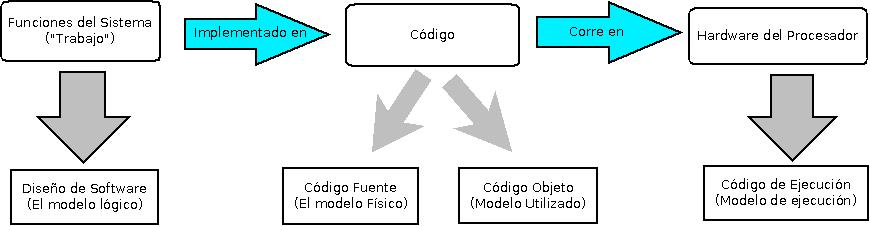
\includegraphics[width=100mm]{runtime}
\caption{Etapas desde el diseño hasta la ejecución}
\label{cap1:001}
\end{figure}

Primero el diseño del software, resulta en el diseño o modelo lógico. Esto es implementado como código fuente, el modelo físico. El código fuente es compilado, enlazado y construido a un código objeto, el modelo bajado (deployment model). Finalmente el código objeto es cargado en el procesador y despues ejecutado, el modelo de ejecución. 
El modelo del código nos proporciona un visión estática del software. En contraste con el modelo de ejecución, una combinación de código, datos y procesador, representa software en ejecución. Esto se define como un proceso de software, también conocida como una tarea en el mundo de los embebidos. En palabras simples, una tarea representa la ejecución de un programa secuencial simple. Por lo regular al modelo de ejecución también se le llama modelo de tareas.

\begin{figure}
\centering
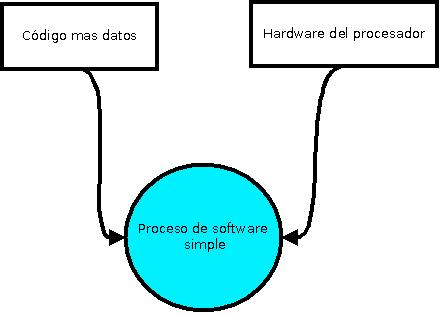
\includegraphics[width=80mm]{runtimemodel}
\caption{El modelo de ejecución del proceso de software}
\label{cap1:002}
\end{figure}

\section{La importancia del tiempo y el temporizado}
En sistemas electrónicos analógicos todas las operaciones pueden, si se requiere, realizarse simultáneamente (concurrentemente), no solamente eso, sino que el procesamiento es hecho instantáneamente. Pero esto no es posible en sistemas basados en procesador ya que este es fundamentalmente discreto en sus operaciones:

\begin{itemize}
	\item Un procesador puede hacer solamente una cosa a tiempo (una maquina secuencial) y
	\item Las operaciones toman tiempo - las cosas no suceden instantáneamente
\end{itemize}

Estos son dos factores que causan muchas angustias en nuestro trabajo de diseño. Y esta es la razón por lo cual si esta diseñando sin conocer tus necesidades de tiempo, debes estar preparado para sorpresas desagradables.

Con esto en mente, los primeros diseños tenían las siguientes características:
\begin{itemize}
	\item Es ejecutado en un lazo continuo
	\item Termina su trabajo en cada lazo (Semantica de ejecutar hasta completar)
	\item Toma tiempo para completar su trabajo (Tiempo de ejecución de tareas- $Te$)
	\item Es repetido a intervalos regulares o periodos (operaciones periodicas - $Tp$)
	\item No hacer nada mientras esta retardado (tiempo desperdiciado $Ts$)
	\item Necesita un mecanismo de temporizado para controlar el periodo de tiempo 
\end{itemize}

En este diseño en particular $Tp$ y $Td$ son requisitos del sistema, $Te$ depende de nuestro código de solución y $Ts$ es nuestro tiempo limite, como puede verse en la figura . Por ejemplo, suponiendo que $Tp$ es $100ms$ y $Te$ es $5ms$, esto nos da un valor de $Ts$ de $95ms$. Esto quiere decir que el procesador esta ejecutando código por $5ms$ cada $100ms$, una utilización ($U$) de $5$\%. 

\begin{figure}
\centering
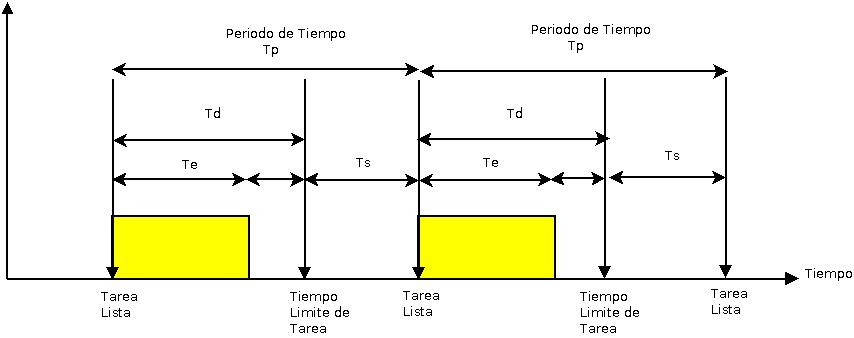
\includegraphics[width=100mm]{timing}
\caption{Algunas definiciones básicas del Temporizado de Tareas}
\label{cap1:003}
\end{figure}
Primero, en los sistemas embebidos se pretende que las tareas se ejecuten hasta ser completadas cada vez que sean activadas. Segundo, en los sitemas prácticos debe haber un tiempo de espera $Ts$. Tercero, por el hecho de que un código se pueda ejecutar dentro de un periodo de tiempo esto no significa que su rendimiento sea aceptable. El retardo de tiempo del procesamiento de entrada-salida puede causar problemas en el comportamiento de todo el sistema.


\section{Manejando múltiples trabajos}
Para manejar trabajos concurrentes independientes, lo cual significa que tenemos diferentes trabajos que en el mundo real pueden:
\begin{enumerate}
	\item Ser atendidos a intervalos regulares - Funciones periódicas
	\item Ser atendidos en tiempos aleatorios - Funciones asíncronas o aperiodicas
	\item Ser procesados simultaneamente
	\item Muy diferentes necesidades de temporizado
\end{enumerate}

\section{Usando Interrupciones como máquina de ejecución}

Un \textbf{timer} se dispara, un interruptor se presiona, un dispositivo periférico necesita atención, son eventos típicos del mundo real en sistemas basados en computadoras. Hay, de hecho, solamente dos maneras de detectar estos eventos: Buscando estos eventos (polling) o enviando una señal directamente a el procesador (interrupciones de hardware).

A diferencia de los métodos anteriores cuando se usaba el polling dentro de una unidad secuencial de programa, ahora se buscan las interrupciones de hardware, una señal electrónica que es aplicada al procesador. Cuando la interrupción es generada se llama a una respuesta predeterminada (la cual es predefinida por el programador)  para ejecutar un software específico. Así que la interrupción puede ser vista como una máquina de ejecución de una pieza particular de software.

Así que lo que tenemos es una ejecución aparentemente concurrente de un conjunto individual de procesos (tareas), llamado ``cuasi-concurrencia''. En otras palabras, usando interrupciones, podemos correr múltiples tareas simultáneamente: una forma de multitareas simple. De esta forma se puede concluir que:

\begin{enumerate}
	\item Las interrupciones son mecanismos habilitados por llaves que permiten al diseño trabajar
	\item Las interrupciones simplifican el diseño funcional del sistema
	\item Las interrupciones simplifican el manejo de diferentes temporizados y requisitos de respuestas
	\item El comportamiento actual en tiempo de ejecución no puede ser predicho o analizado estáticamente
\end{enumerate}

\bibliographystyle{acm}
\bibliography{../bibliografia}
\end{document}